\section{lib/efreet\_\-private.h File Reference}
\label{efreet__private_8h}\index{lib/efreet\_\-private.h@{lib/efreet\_\-private.h}}


\subsection{Detailed Description}
Contains methods and defines that are private to the Efreet implementaion. 



{\tt \#include \char`\"{}config.h\char`\"{}}\par
{\tt \#include $<$stdlib.h$>$}\par
{\tt \#include $<$stdio.h$>$}\par
{\tt \#include $<$string.h$>$}\par
{\tt \#include $<$unistd.h$>$}\par
{\tt \#include $<$ctype.h$>$}\par
{\tt \#include $<$fcntl.h$>$}\par
{\tt \#include $<$sys/mman.h$>$}\par
{\tt \#include $<$sys/types.h$>$}\par
{\tt \#include $<$sys/stat.h$>$}\par
{\tt \#include $<$dirent.h$>$}\par
{\tt \#include $<$fnmatch.h$>$}\par
{\tt \#include $<$limits.h$>$}\par
{\tt \#include $<$Eina.h$>$}\par
{\tt \#include $<$Ecore.h$>$}\par
{\tt \#include $<$Ecore\_\-File.h$>$}\par
{\tt \#include $<$Ecore\_\-Str.h$>$}\par
{\tt \#include \char`\"{}efreet\_\-xml.h\char`\"{}}\par
{\tt \#include \char`\"{}efreet\_\-ini.h\char`\"{}}\par


Include dependency graph for efreet\_\-private.h:\nopagebreak
\begin{figure}[H]
\begin{center}
\leavevmode
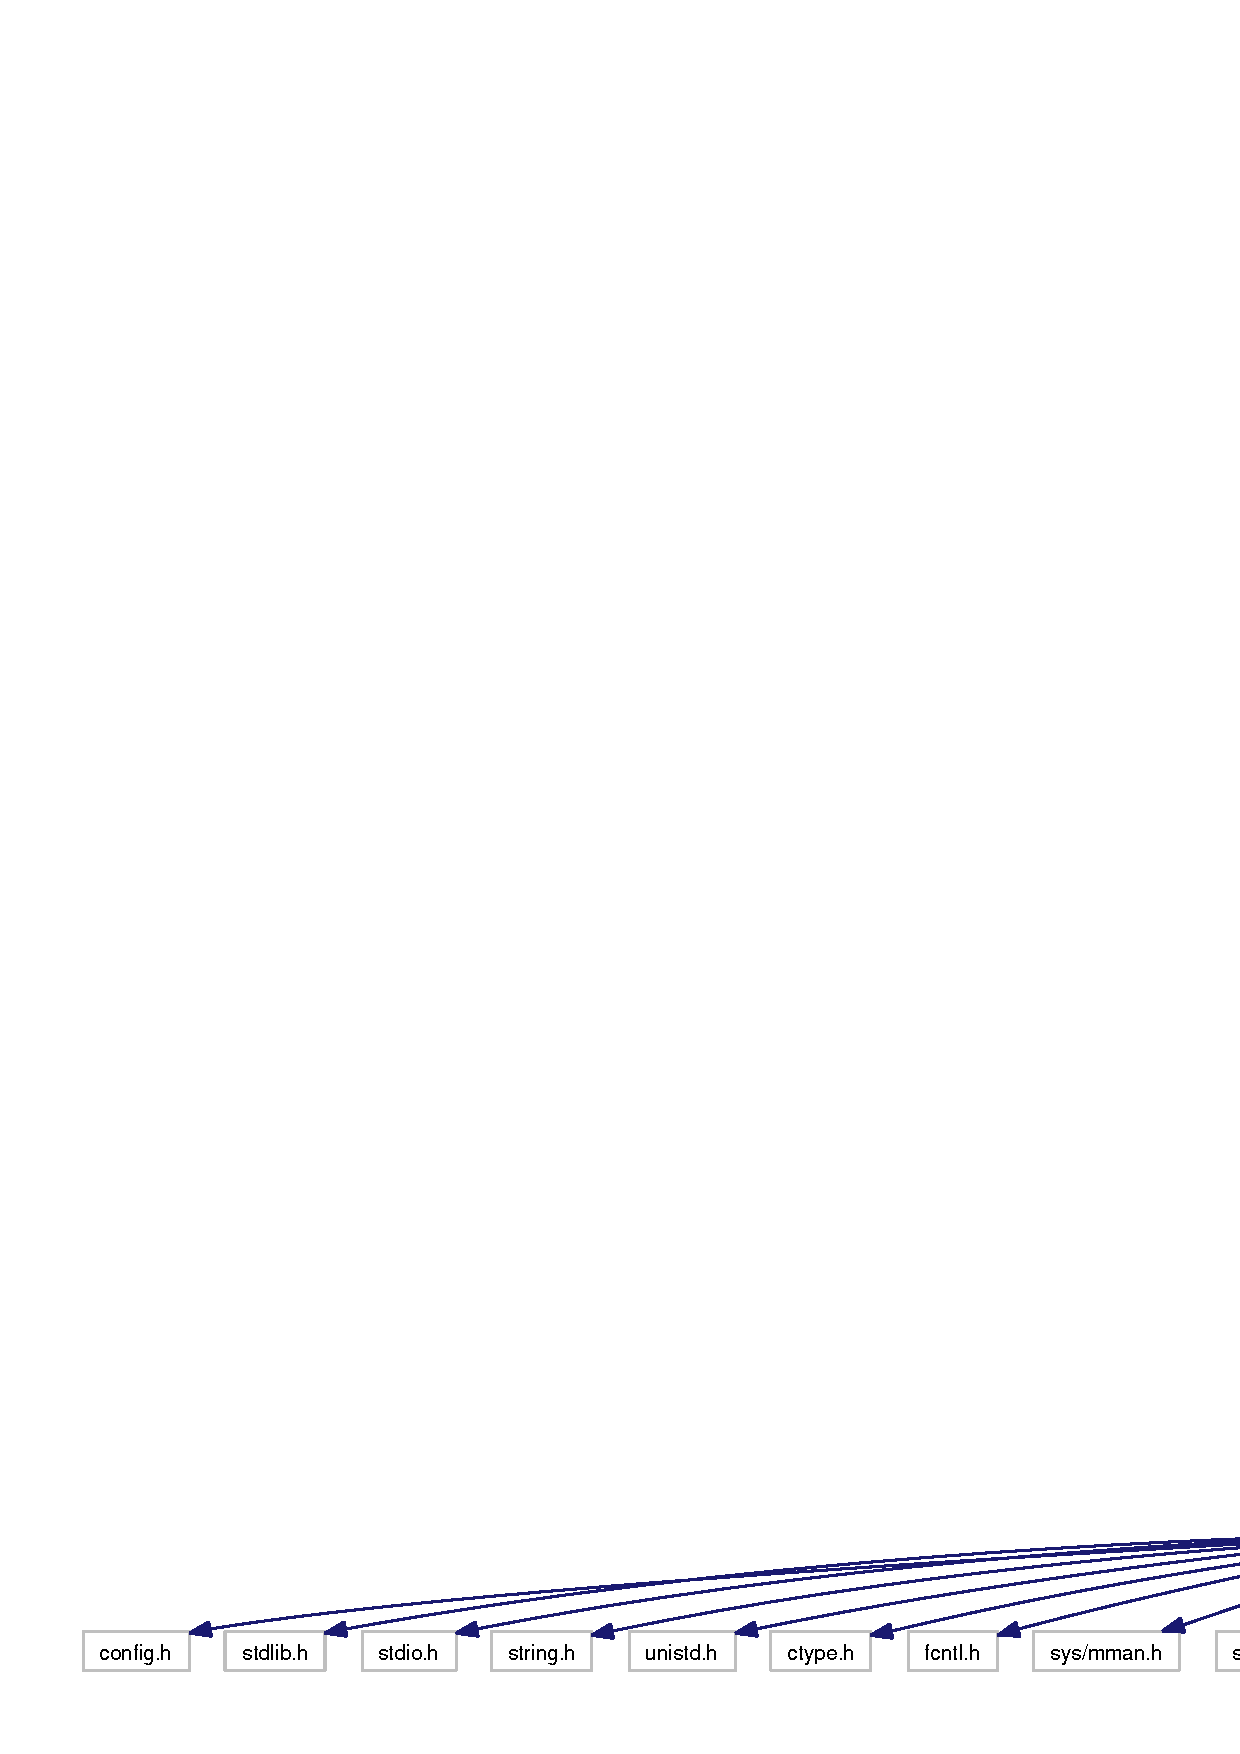
\includegraphics[width=420pt]{efreet__private_8h__incl}
\end{center}
\end{figure}


This graph shows which files directly or indirectly include this file:\nopagebreak
\begin{figure}[H]
\begin{center}
\leavevmode
\includegraphics[width=420pt]{efreet__private_8h__dep__incl}
\end{center}
\end{figure}
\subsection*{Data Structures}
\begin{CompactItemize}
\item 
struct {\bf Efreet\_\-Desktop\_\-Command}
\item 
struct {\bf Efreet\_\-Desktop\_\-Command\_\-File}
\end{CompactItemize}
\subsection*{Defines}
\begin{CompactItemize}
\item 
\#define {\bf FREE}(x)~do \{ free(x); x = NULL; \} while (0)
\item 
\#define {\bf IF\_\-FREE}(x)~do \{ if (x) FREE(x); \} while (0)
\item 
\#define {\bf IF\_\-FREE\_\-DLIST}(x)
\item 
\#define {\bf IF\_\-FREE\_\-HASH}(x)
\item 
\#define {\bf IF\_\-FREE\_\-LIST}(x)
\item 
\#define {\bf IF\_\-RELEASE}(x)
\item 
\#define {\bf NEW}(x, c)~calloc(c, sizeof(x))
\item 
\#define {\bf PATH\_\-MAX}~4096
\end{CompactItemize}
\subsection*{Typedefs}
\begin{CompactItemize}
\item 
typedef struct {\bf Efreet\_\-Desktop\_\-Command} {\bf Efreet\_\-Desktop\_\-Command}
\item 
typedef struct {\bf Efreet\_\-Desktop\_\-Command\_\-File} {\bf Efreet\_\-Desktop\_\-Command\_\-File}
\item 
typedef enum {\bf Efreet\_\-Desktop\_\-Command\_\-Flag} {\bf Efreet\_\-Desktop\_\-Command\_\-Flag}
\end{CompactItemize}
\subsection*{Enumerations}
\begin{CompactItemize}
\item 
enum {\bf Efreet\_\-Desktop\_\-Command\_\-Flag} \{ {\bf EFREET\_\-DESKTOP\_\-EXEC\_\-FLAG\_\-FULLPATH} =  0x0001, 
{\bf EFREET\_\-DESKTOP\_\-EXEC\_\-FLAG\_\-URI} =  0x0002, 
{\bf EFREET\_\-DESKTOP\_\-EXEC\_\-FLAG\_\-DIR} =  0x0004, 
{\bf EFREET\_\-DESKTOP\_\-EXEC\_\-FLAG\_\-FILE} =  0x0008
 \}
\end{CompactItemize}
\subsection*{Functions}
\begin{CompactItemize}
\item 
size\_\-t {\bf efreet\_\-array\_\-cat} (char $\ast$buffer, size\_\-t size, const char $\ast$strs[$\,$])
\item 
int {\bf efreet\_\-base\_\-init} (void)
\item 
void {\bf efreet\_\-base\_\-shutdown} (void)
\item 
Ecore\_\-List $\ast$ {\bf efreet\_\-default\_\-dirs\_\-get} (const char $\ast$user\_\-dir, Ecore\_\-List $\ast$system\_\-dirs, const char $\ast$suffix)
\begin{CompactList}\small\item\em Creates the list of directories based on the user dir, system dirs and given suffix. \item\end{CompactList}\item 
const char $\ast$ {\bf efreet\_\-desktop\_\-environment\_\-get} (void)
\begin{CompactList}\small\item\em sets the global desktop environment name \item\end{CompactList}\item 
int {\bf efreet\_\-desktop\_\-init} (void)
\item 
int {\bf efreet\_\-desktop\_\-shutdown} (void)
\item 
const char $\ast$ {\bf efreet\_\-home\_\-dir\_\-get} (void)
\item 
int {\bf efreet\_\-icon\_\-init} (void)
\item 
void {\bf efreet\_\-icon\_\-shutdown} (void)
\item 
int {\bf efreet\_\-ini\_\-init} (void)
\item 
int {\bf efreet\_\-ini\_\-shutdown} (void)
\item 
EAPI const char $\ast$ {\bf efreet\_\-lang\_\-country\_\-get} (void)
\item 
EAPI const char $\ast$ {\bf efreet\_\-lang\_\-get} (void)
\item 
EAPI const char $\ast$ {\bf efreet\_\-lang\_\-modifier\_\-get} (void)
\item 
int {\bf efreet\_\-menu\_\-init} (void)
\begin{CompactList}\small\item\em Initializes the Efreet Menu system. \item\end{CompactList}\item 
void {\bf efreet\_\-menu\_\-shutdown} (void)
\begin{CompactList}\small\item\em Shuts down the Efreet menu system. \item\end{CompactList}\end{CompactItemize}
